\chapter{Opis projektnog zadatka}
			
		Projektni zadatak jest razvoj programske podrške za ostvarenje mrežne aplikacije BytePit. Aplikacija predstavlja platformu za rješavanje programerskih zadataka i provođenje natjecanja u programiranju. Aplikacija BytePit  pruža ključne mogućnosti kao što su:
		\begin{itemize}
			\item \textit{registracija natjecatelja i voditelja natjecanja}
			\item \textit{dijeljenje osmišljenih zadataka iz natjecateljskog programiranja}
			\item \textit{rješavanje zadataka i evaluacija rješenja na temelju testnih primjera}
			\item \textit{kreiranje i provođenje natjecanja.}
		\end{itemize}
		
		Zbog ovih je mogućnosti aplikacija BytePit od posebnog interesa za odgojno-obrazovne ustanove koje alat mogu koristiti kao dodatak u nastavi predmeta povezanih uz programiranje (provođenje ispita ili domaćih zadaća), sudionike natjecanja u programiranju koji na platformi mogu u slobodno vrijeme vježbati i usavršavati svoje vještine te udruge i druga tijela koja se bave organizacijom natjecanja iz programiranja ili pak promocijom računalne znanosti. IT kompanije bi ovu aplikaciju mogle upotrebljavati kako bi ispitale relevantna znanja i programerske sposobnosti potencijalnih novih zaposlenika.
		
		Aplikacija na početnoj stranici mora nuditi mogućnost registracije novim korisnicima. Proces registracije, uz mogućnost odabira uloge (voditelj natjecanja ili natjecatelj), zahtijeva unos korisničkog imena, fotografije, lozinke, imena, prezimena i adrese e-pošte. Za završetak registracije potrebno je otvoriti poveznicu dobivenu putem e-pošte. Voditeljevu registraciju mora dodatno odobriti administrator, koji pored toga ima ovlasti za upravljanje registriranim korisnicima i njihovim podacima, uključujući dodjelu prava i promjene osobnih podataka.
		
		Tri su osnovna tipa korisnika aplikacije:
		\begin{itemize}
			\item \textbf{natjecatelji} --- Natjecatelji su osnovni korisnici aplikacije i njezina glavna ciljna skupina. Osnovne usluge koje im se pružaju su sudjelovanje u programerskim natjecanjima, rješavanje zadataka i praćenje svog napretka. Na zahtjev mogu pristupiti zadacima (tijekom ili izvan termina natjecanja) . Mogu slati programska rješenja na evaluaciju, a nakon natjecanja pratiti i rangiranje s obzirom na ostale natjecatelje. Na profilima natjecatelja, vidljive su različite statistike, uključujući broj točno riješenih zadataka, broj pokušaja rješavanja zadataka te prikaz osvojenih pehara za natjecanja. Natjecatelji mogu organizirati i virtualna natjecanja, koja se temelje na prošlim natjecanjima u kalendaru. Ta natjecanja su aktivna samo za njih, a rangiraju se prema službenim rezultatima originalnih natjecanja. Također, mogu kreirati virtualna natjecanja s nasumično odabranim zadacima, ravnomjerno raspoređenim prema težini zadataka.
 			\item \textbf{voditelji} --- Voditelji natjecanja organiziraju i upravljaju programerskim natjecanjima na platformi. To uključuje postavljanje natjecanja, dodavanje zadataka i praćenje rezultata sudionika. Prilikom kreiranja novih natjecanja moraju postaviti parametre, kao što su datum objave i trajanje natjecanja, dodati zadatke i po želji slike pehara. Dodavanje programerskih zadataka u natjecanja uključuje i postavljanje njihovih karakteristika -- bodova i vremenskog ograničenja, ali i testnih primjera. Profili voditelja sadrže popis zadataka koje su učitali, s mogućnošću sortiranja.
			\item \textbf{administratori} --- Administratori imaju ovlasti za upravljanje cijelom platformom, uključujući i korisničke račune. Upravljanje registriranim korisnicima i njihovim podacima uključuje dodjelu prava (primjerice potvrdu registracije voditelja) i promjene osobnih podataka korisnika. Administrator ima ovlasti za uređivanje svih zadataka i natjecanja pri čemu se se ne mijenjaju prethodno ostvareni rezultati.
		\end{itemize}
		
		Središnji dijelovi aplikacije su \emph{zadaci} i \emph{natjecanja}. Programerski zadaci su ključna komponenta aplikacije i pružaju izazove korisnicima koji žele razvijati svoje programerske sposobnosti. Svaki zadatak dolazi s nazivom, jedinstvenim opisom, brojem bodova koji se mogu osvojiti i vremenskim ograničenjem za rješavanje. Zadatak može biti postavljen kao privatan ili javan, a svaki privatni zadatak dodan u natjecanje, po završetku istog, postaje javan. Natjecatelji biraju zadatke koji ih zanimaju (ili koji su dio natjecanja) i šalju svoje rješenje u obliku izvornog programskog koda. Evaluacija rješenja (omogućena samo za jedan programski jezik) temelji se na usporedbi generiranih izlaza programa s očekivanim izlazima iz testnih primjera. Dodijeljeni broj bodova proporcionalan je postotku točnih primjera. Za svaki zadatak dostupan je popis svih natjecatelja koji su poslali rješenje za taj zadatak. Ovaj popis sadrži informacije o broju točno riješenih primjera, prosječnom vremenu izvršavanja po primjeru te omogućava pristup učitanim rješenjima. Važno je napomenuti da opcija za pristup učitanim rješenjima aktivira samo za one natjecatelje koji su uspješno i potpuno riješili zadatak.
		
		Natjecanja predstavljaju srce platforme, potičući korisnike da pokažu svoje programerske vještine i natječu se s drugima. Voditelji natjecanja imaju ključnu ulogu u organizaciji ovih događaja. Oni kreiraju i definiraju ključne elemente natjecanja. Natjecatelji se prijavljuju za sudjelovanje u natjecanjima, a tijekom trajanja rješavaju zadatke i šalju svoja rješenja. Početkom natjecanja prijavljeni natjecatelji mogu pristupiti svim zadacima koji se nalaze u njemu. Nakon završetka natjecanja, rezultati se prikazuju na profilima natjecatelja, a osvajači pehara nagrađuju se za svoje uspjehe. Također, natjecatelji imaju mogućnost pregledavanja svih rješenja koja su drugi natjecatelji poslali za isti zadatak.
		
		Rješenje za ovu aplikaciju biti će ostvareno pomoću razvojnog okvira Springboota i JavaScript biblioteka React kojom će biti modelirano korisničko sučelje.
		
		Moguća poboljšanja za aplikaciju BytePit uključuju unaprjeđenje korisničkog sučelja radi olakšane navigacije, uvođenje ocjena i komentara za zadatke i natjecanja, implementaciju sustava za korisničku komunikaciju putem chatova ili foruma, bolje statističke podatke i analitiku na korisničkim profilima, integraciju s razvojnim alatima, raznolikost vrsta zadataka, napredniju evaluaciju rješenja s podrškom za različite programske jezike, te dodatak edukativnih materijala kako bi se potaknulo učenje i razvoj programerskih vještina među korisnicima. 
		
Primjeri sličnih rješenja kroz koje ćemo proći su:
		\begin{itemize}
			\item \textit{Edgar}
			\item \textit{Sphere online judge}
			\item \textit{Codeforces}
		\end{itemize}
		
		Kao i u sustavima \emph{Edgar, SPOJ i Codeforces}, korisnici će moći pregledavati zadatke na stranici, te će moći na svom profilu vidjeti statistiku u odnosu na preostale natjecatelje, te svoj rank. Također mogu na kalendaru vidjeti vrijeme odvijanja budućih natjecanja. 
		
		\begin{figure}[H]
			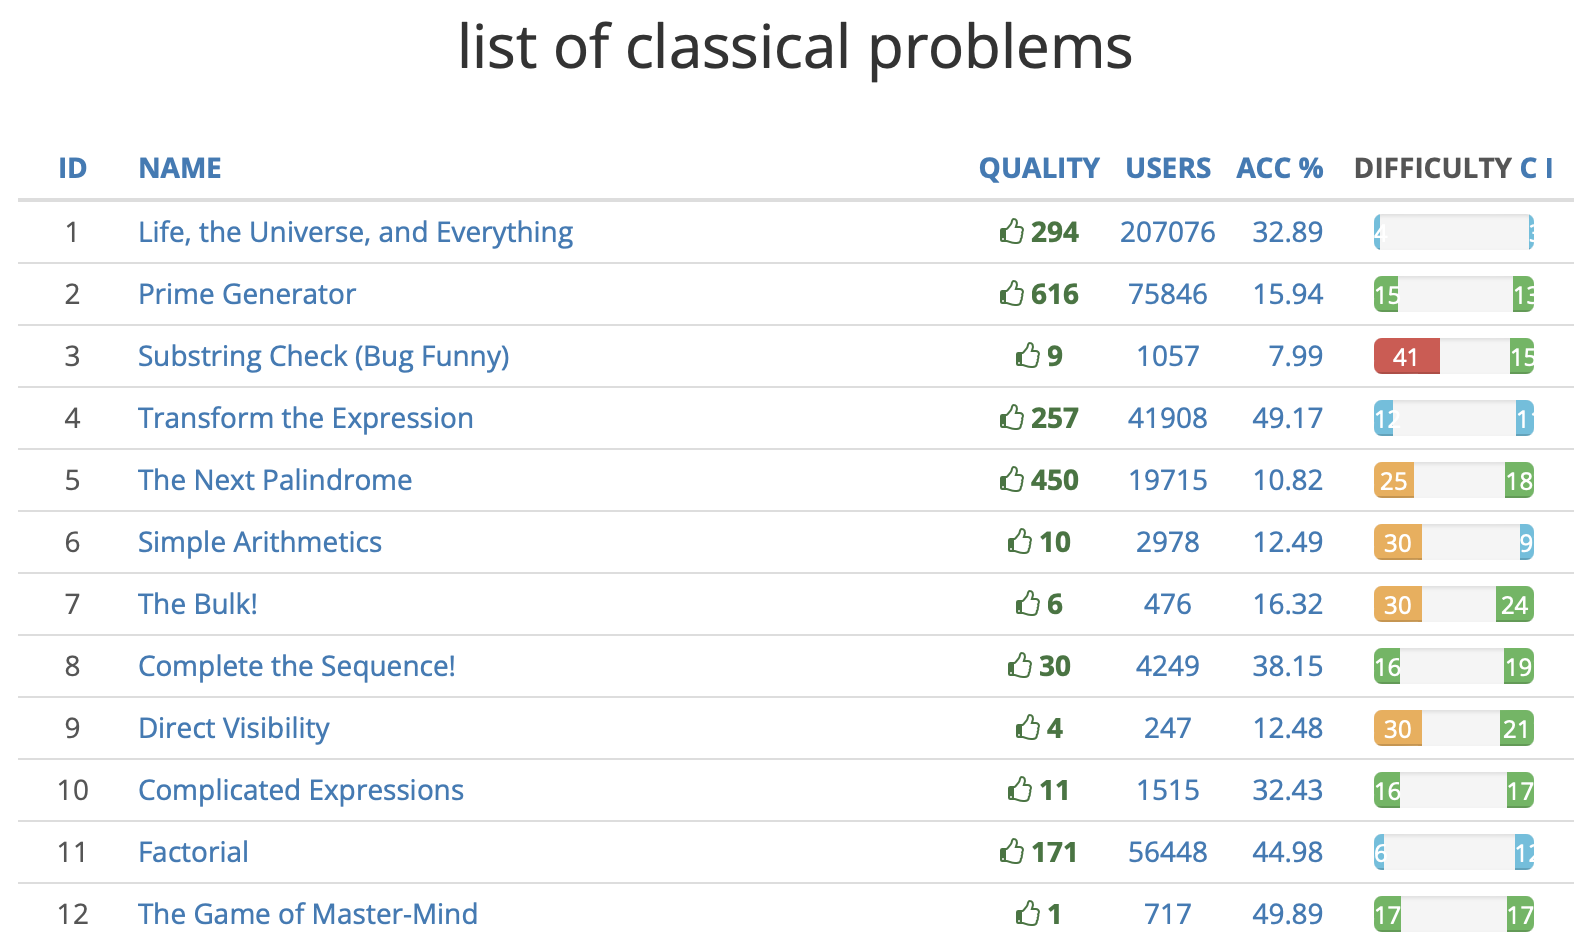
\includegraphics[scale=0.4]{slike/spoj1.png}
			\centering
			\caption{Sustav SPOJ - pregled zadataka na stranici}
			\label{fig:spoj1}
		\end{figure}
		
		\begin{figure}[H]
			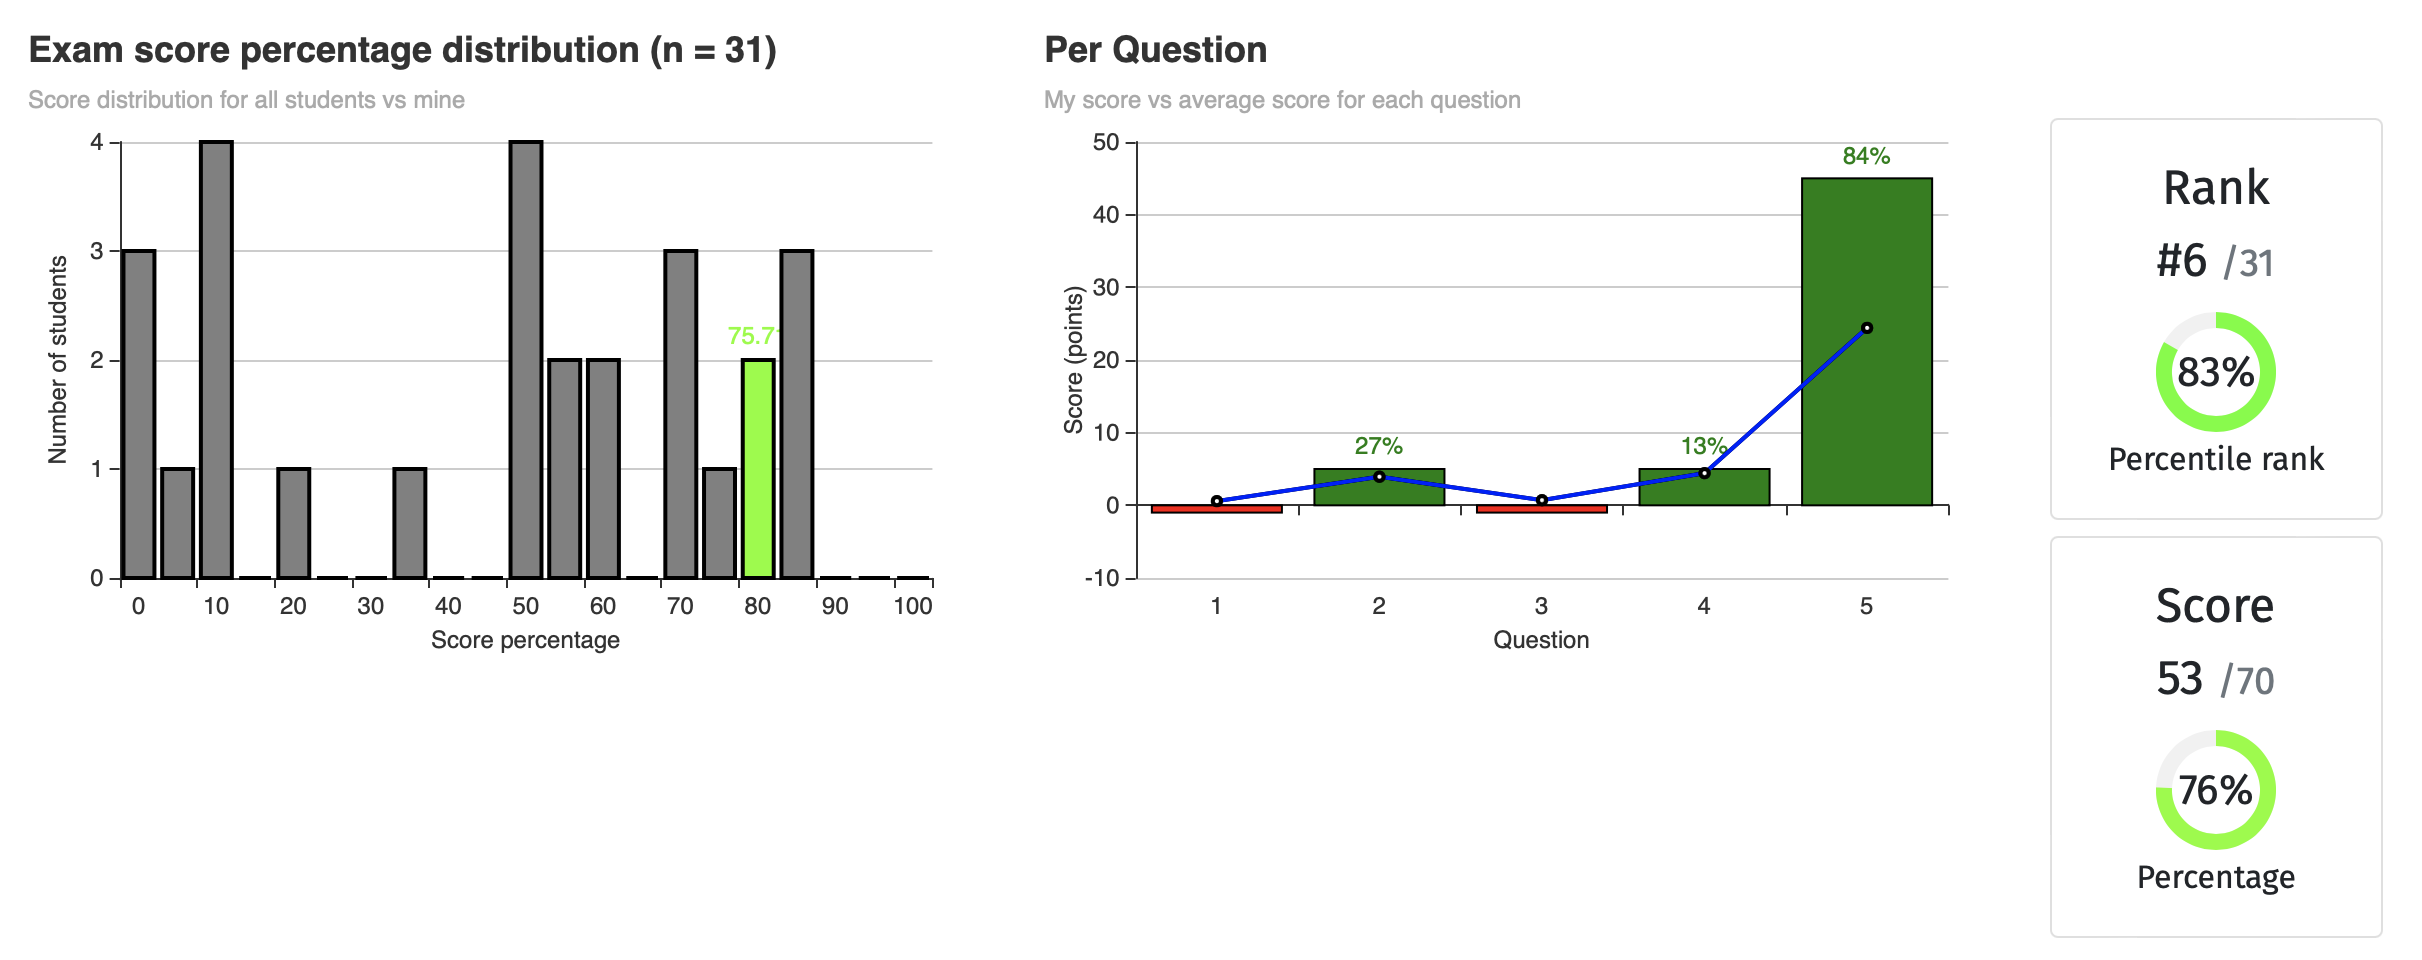
\includegraphics[scale=0.4]{slike/edgar2.png}
			\caption{Sustav Edgar - pregled statistike ispita}
			\label{fig:edgar2}
		\end{figure}
		
		\begin{figure}[H]
			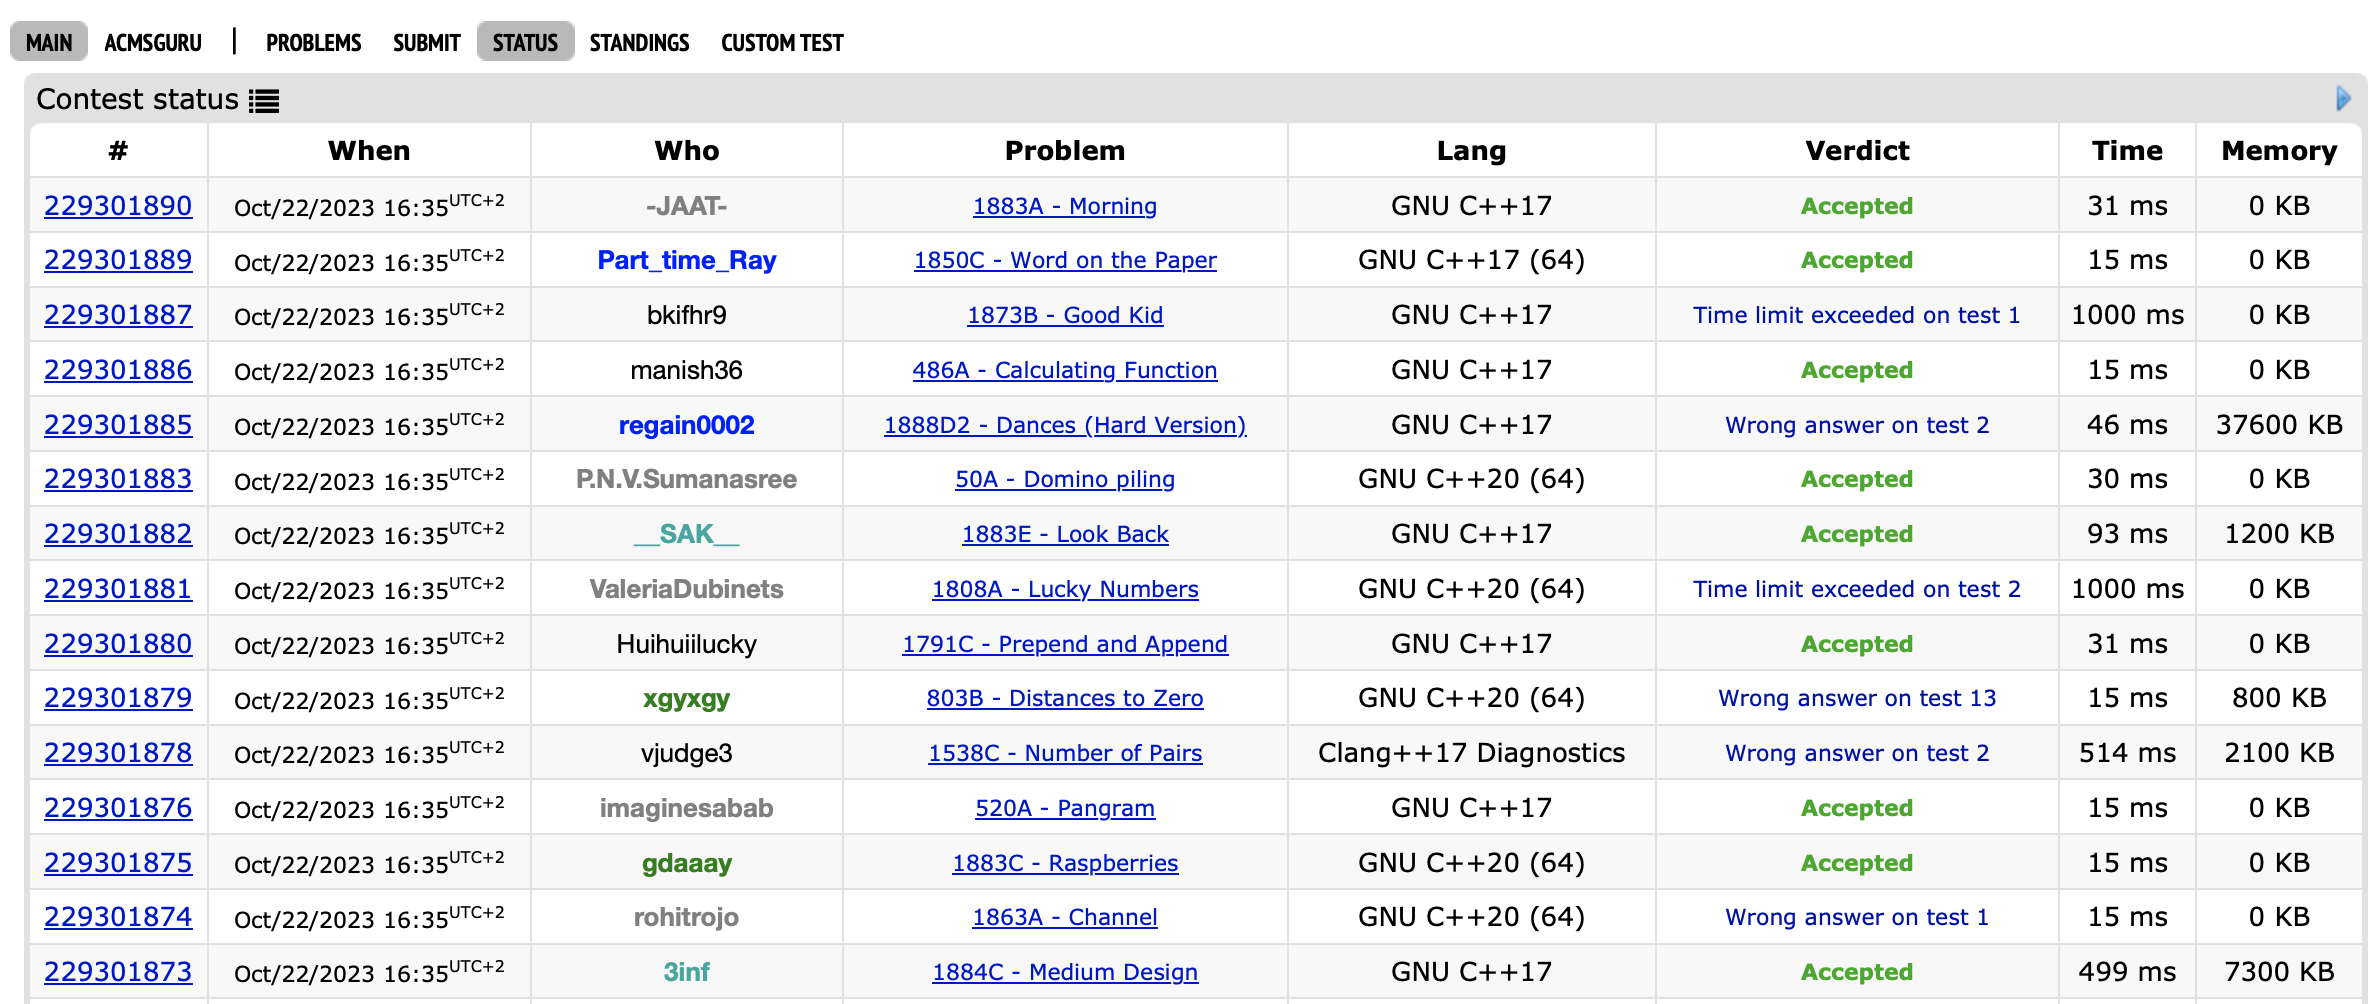
\includegraphics[scale=0.4]{slike/codeforces1.png} 
			\centering
			\caption{Sustav Codeforces - pregled statusa na natjecanju}
			\label{figure:codeforces1}
		\end{figure}
		
		\begin{figure}[H]
			
\includegraphics[scale=0.4]{slike/codeforces2.png} 
			\centering
			\caption{Sustav Codeforces - kalendar nadolazećih natjecanja}
			\label{fig:codeforces2}
		\end{figure}
		
		Ukoliko natjecatelja zanima profil nekog drugog natjecatelja, klikom na ime profila će se otvoriti stranica na kojoj je moguće vidjeti statistiku natjecatelja: broj točno rješenih zadataka, pehari, broj svih pokrenutih zadataka. \emph{Codeforces} dodatno daje prikaz aktivnosti natjecatelja u vremenskom periodu od jedne godine.
		
		\begin{figure}[H]
			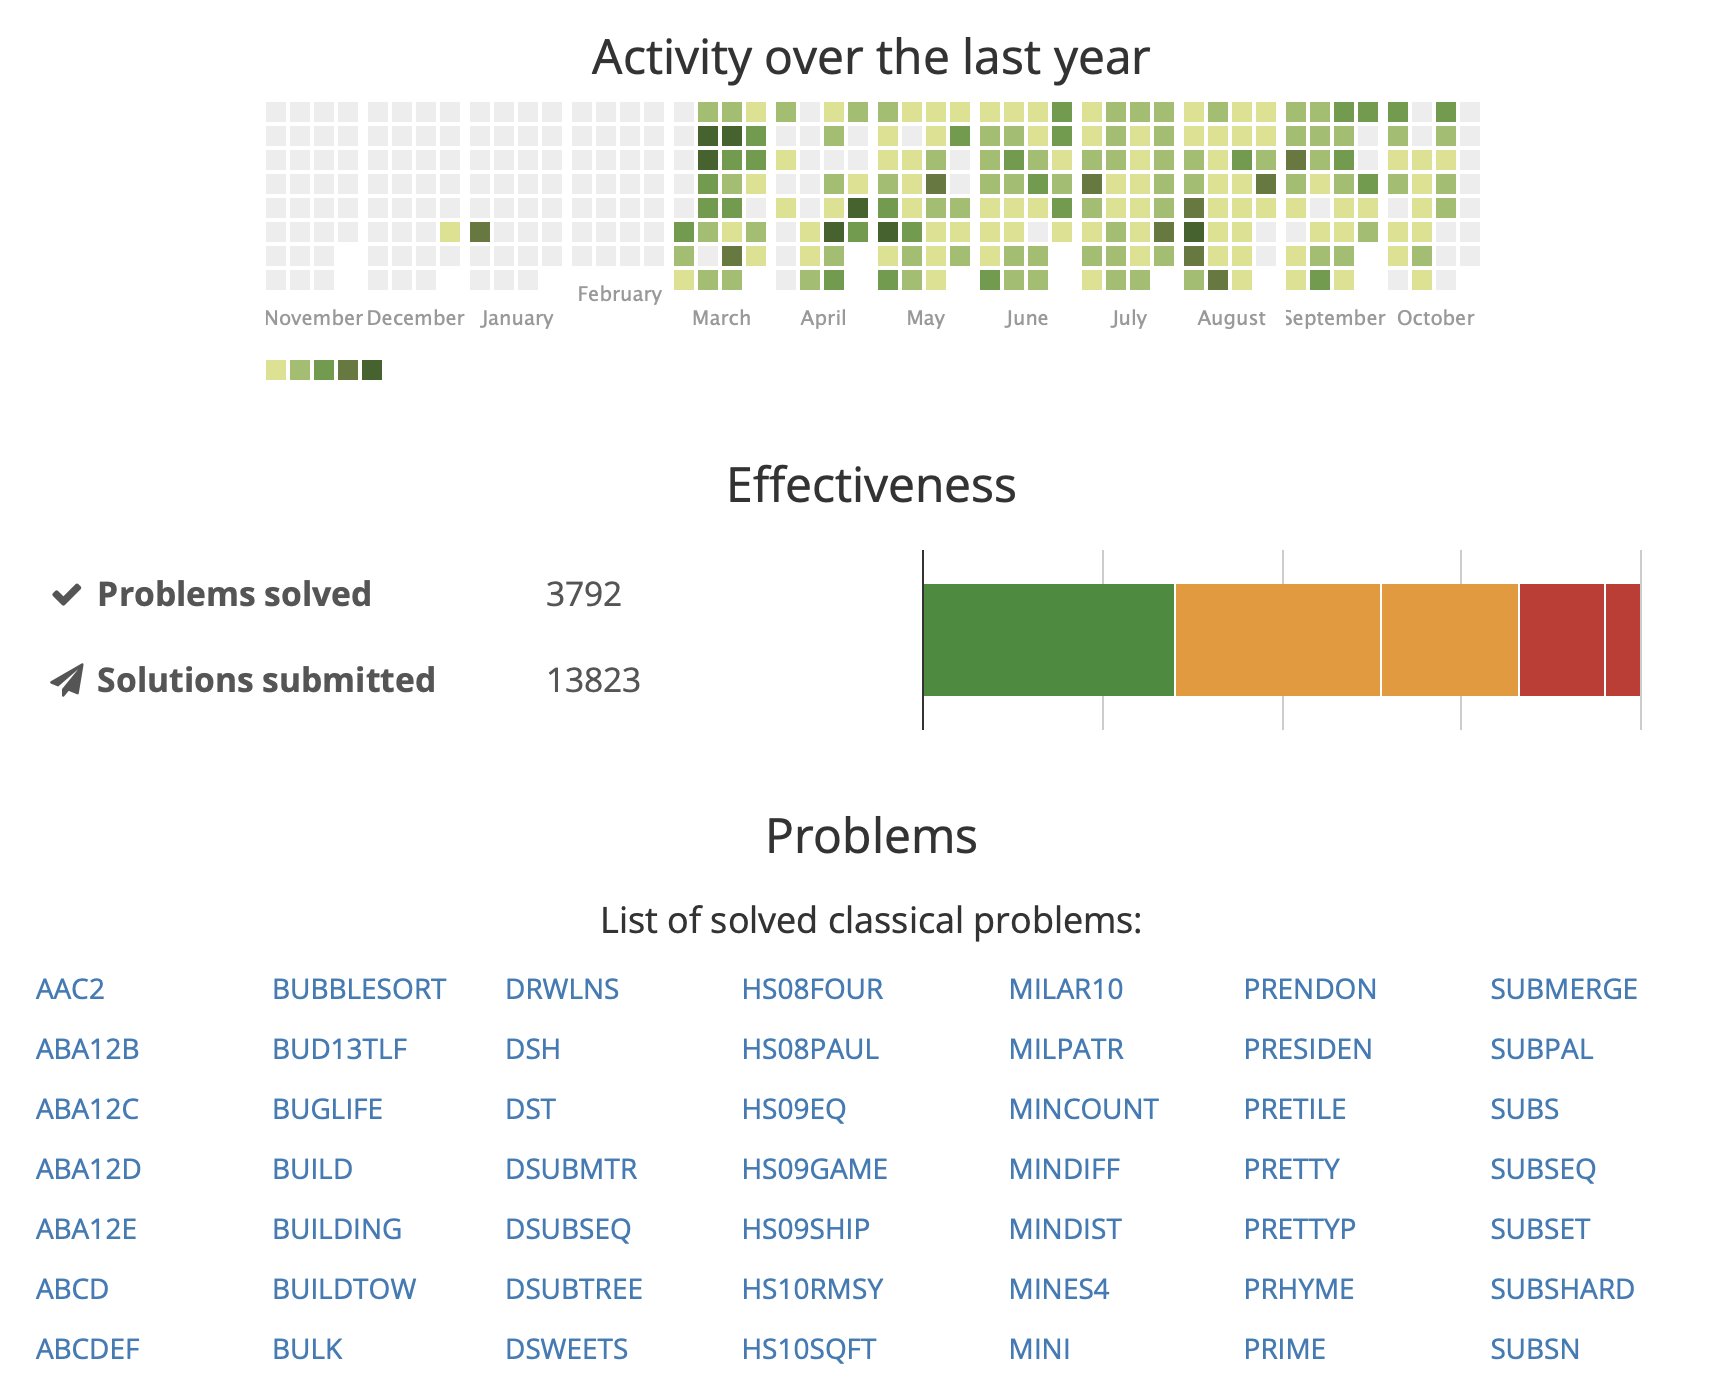
\includegraphics[scale=0.4]{slike/spoj2.png} 
			\centering
			\caption{Sustav SPOJ - profil natjecatelja}
			\label{fig:spoj2}
		\end{figure}		
		
	
